\documentclass{article}
\usepackage[utf8]{inputenc}
\usepackage{graphicx} % Required for inserting images
\usepackage{hyperref}
\usepackage{subcaption}
\usepackage{float}
\usepackage{tcolorbox}
\usepackage{amsmath}
\usepackage{amssymb}
\usepackage{listings}% http://ctan.org/pkg/listings}
\usepackage{algorithm}
\usepackage{algorithmic}
\usepackage[toc,page]{appendix}
\usepackage[backend=biber]{biblatex}
\usepackage{multicol}
\usepackage{siunitx}
\usepackage{comment}
\usepackage{xcolor}
\usepackage{caption}
\usepackage{tikz}
\usetikzlibrary{shapes.geometric, arrows}

\tikzstyle{startstop} = [rectangle, rounded corners, 
minimum width=3cm, 
minimum height=1cm,
text centered, 
draw=black, 
fill=red!30]

\tikzstyle{io} = [trapezium, 
trapezium stretches=true, % A later addition
trapezium left angle=70, 
trapezium right angle=110, 
minimum width=3cm, 
minimum height=1cm, text centered, 
draw=black, fill=blue!30]

\tikzstyle{process} = [rectangle, 
minimum width=3cm, 
minimum height=1cm, 
text centered, 
text width=3cm, 
draw=black, 
fill=orange!30]

\tikzstyle{decision} = [diamond, 
minimum width=3cm, 
minimum height=1cm, 
text centered, 
draw=black, 
fill=green!30]
\tikzstyle{arrow} = [thick,->,>=stealth]

% To delete lstlisting caption "Listing x"
%\captionsetup[lstlisting]{labelformat=empty}

\lstdefinestyle{myStyle}{
    belowcaptionskip=1\baselineskip,
    breaklines=true,
    frame=none,
    numbers=none, 
    basicstyle=\footnotesize\ttfamily,
    keywordstyle=\bfseries\color{green!40!black},
    commentstyle=\itshape\color{purple!40!black},
    identifierstyle=\color{black},
    backgroundcolor=\color{white},
}

\lstdefinestyle{cypherStyle}{
    backgroundcolor=\color{white},   % choose the background color
    basicstyle=\footnotesize\ttfamily,        % the size of the fonts that are used for the code
    commentstyle=\itshape\color{purple!40!black},
    keywordstyle=\bfseries\color{green!40!black},
    breakatwhitespace=false,         % sets if automatic breaks should only happen at whitespace
    breaklines=true,                 % sets automatic line breaking
    captionpos=b,                    % sets the caption-position to bottom
    commentstyle=\color{gray},    % comment style
    deletekeywords={},            % if you want to delete keywords from the given language
    escapeinside={\%*}{*)},          % if you want to add LaTeX within your code
    extendedchars=true,              % lets you use non-ASCII characters; for 8-bits encodings only, does not work with UTF-8
    %firstnumber=1000,                % start line enumeration with line 1000
    frame=none,                    % adds a frame around the code
    keepspaces=true,                 % keeps spaces in text, useful for keeping indentation of code (possibly needs columns=flexible)
    language=SQL,                    % the language of the code
    morekeywords={*,IF, REQUIRE, FOR, IS, LOAD, CSV, WITH, HEADERS, MERGE, toFloat, toInteger, date},            % if you want to add more keywords to the set
    numbers=none,                    % where to put the line-numbers; possible values are (none, left, right)
    numbersep=5pt,                   % how far the line-numbers are from the code
    numberstyle=\tiny\color{mygray}, % the style that is used for the line-numbers
    rulecolor=\color{black},         % if not set, the frame-color may be changed on line-breaks within not-black text (e.g. comments (green here))
    showspaces=false,                % show spaces everywhere adding particular underscores; it overrides 'showstringspaces'
    showstringspaces=false,          % underline spaces within strings only
    showtabs=false,                  % show tabs within strings adding particular underscores
    stepnumber=1,                    % the step between two line-numbers. If it's 1, each line will be numbered
    stringstyle=\ttfamily,     % string literal style
    tabsize=2,                       % sets default tabsize to 2 spaces
}

%% Golang definition for listings
%% http://github.io/julienc91/lstlistings-golang
%%
\lstdefinelanguage{Golang}%
  {morekeywords=[1]{package,import,func,type,struct,return,defer,panic,%
     recover,select,var,const,iota,},%
   morekeywords=[2]{string,uint,uint8,uint16,uint32,uint64,int,int8,int16,%
     int32,int64,bool,float32,float64,complex64,complex128,byte,rune,uintptr,%
     error,interface},%
   morekeywords=[3]{map,slice,make,new,nil,len,cap,copy,close,true,false,%
     delete,append,real,imag,complex,chan,},%
   morekeywords=[4]{for,break,continue,range,go,goto,switch,case,fallthrough,if,%
     else,default,},%
   morekeywords=[5]{Println,Printf,Error,Print,},%
   sensitive=true,%
   morecomment=[l]{//},%
   morecomment=[s]{/*}{*/},%
   morestring=[b]',%
   morestring=[b]",%
   morestring=[s]{`}{`},%
}

\lstdefinestyle{golangStyle}{
    captionpos=b,              % sets the caption-position to bottom
    belowcaptionskip=1\baselineskip,
    breaklines=true,
    frame=none,
    numbers=none, 
    basicstyle=\footnotesize\ttfamily,
    keywordstyle=\bfseries\color{green!40!black},
    commentstyle=\itshape\color{purple!40!black},
    identifierstyle=\color{black},
    backgroundcolor=\color{white},
    language=Golang,
}


\title{TFM-FernandoMartín}
\author{Fernando Martín Canfrán}
\date{April 2024}

\begin{document}


\section{Transaction Generator}

First of all it is important to remark that we are first generating ordinary, 
regular transactions that are not fraud kinds of transactions. Therefore the 
transactions generated for each card object have to be generated in such a way
that they will not produce any fraud pattern alert. Later in the process we 
will poison our system by generating those transactions to produce fraud pattern 
alerts.

\subsection{Regular transactions}

Considerations:

\begin{itemize}
  \item Particular ATM usage frequency
  \item ATM selection for the generated transactions of each card
  \item Distribution of the genetated transactions on the decided considered time
\end{itemize}

Some ideas to explore:

\begin{itemize}
  \item ATM - Pre-selection of closed card ATM subset.
  \item Time - Uniform distribution. 
  \item Time - Poisson process distribution.
  \item Random walks.
\end{itemize}

\subsubsection{ATM closed subset + Uniform time distribution}

\begin{itemize}
  \item $\rightarrow$ ATM selection: closed ATM subset.
  \item $\rightarrow$ Time distribution: uniform distribution of the $num\_tx$ transactions 
  for a card on a certain day ($num\_tx$ is drawn from a Poisson distribution of 
  $\lambda = \texttt{withdrawal\_day}$, based on the behavior of the \emph{Wisabi} clients).
\end{itemize}

More detailed explanation follows.
\\


The transaction generator is done to be able to generate transactions for 
each of the cards based on the gathered client transaction behavior of each of the cards 
for a customisable \textcolor{orange}{\texttt{d}} number of days starting in a 
\textcolor{orange}{\texttt{start\_date}}. 

For a card, the idea is to create a certain 
number of transactions per day, by linking the card to a certain ATM that is no farther 
than \textcolor{orange}{\texttt{max\_distance}} kms from the residence location of the 
client of the card. Also, we will limit the time distance between two consecutive 
transactions so that the final set of created transactions can not produce a potential 
fraud related with having two transactions in different ATM locations with an insufficient 
feasible time distance.

For each card:  

\begin{itemize}
    \item \textbf{ATM subset}: Create a subset of ATMs that are considered to be \textit{usual} for 
    the card client, so that they are all at a distance inferior or equal to 
    \textcolor{orange}{\texttt{max\_distance}} kms to the residence location of the client 
    of the card. We limit the size of this subset to be of \textcolor{orange}{\texttt{max\_size\_atm\_subset}}, so that we take only a maximum of \textcolor{orange}{\texttt{max\_size\_atm\_subset}} of the closest ATMs.
    \textcolor{blue}{In addition, among the ATMs in this subset, preference is given to 
    those that are the closest to the residence location of the client and those that 
    belong to the same bank company as the client's card.}
    The transactions generated for this card will be linked only to ATMs of this subset called 
    \texttt{Neighborhood}.

    $$\texttt{Neighborhood} = \{\texttt{ATM}\ | \texttt{dist(ATM, residence\_loc)} \leq \texttt{max\_distance}\}$$

    \begin{figure}[H]
      \centering
      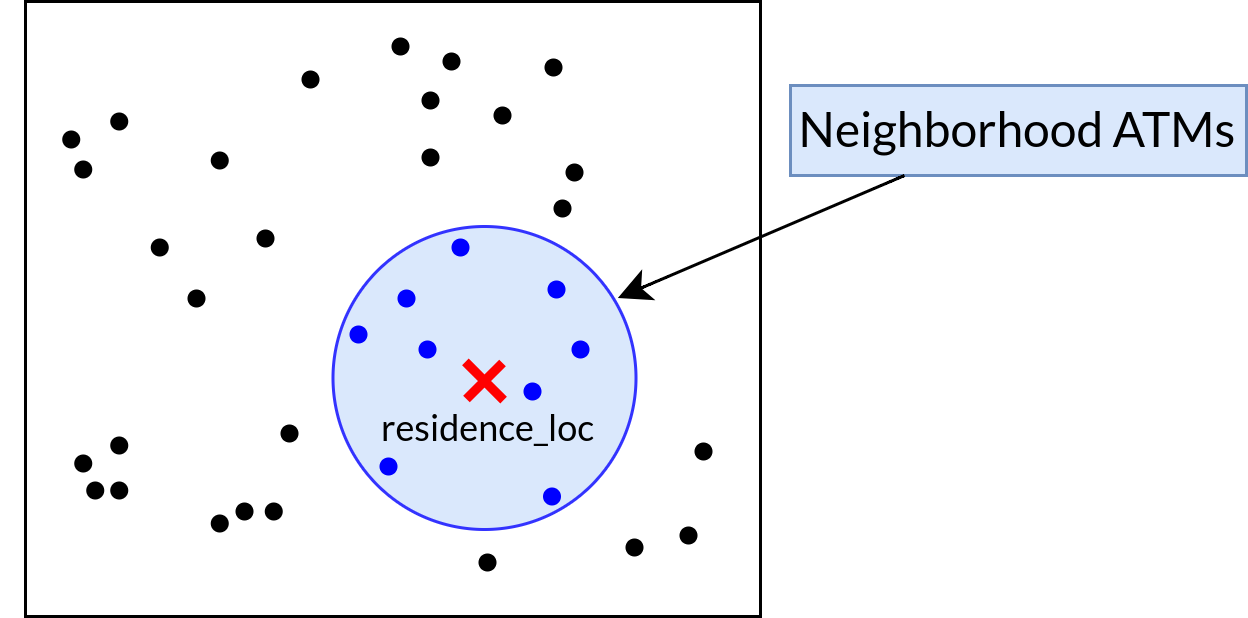
\includegraphics[scale=1.1]{images/tx-generation-1-named.png}
      \caption{\texttt{Neighborhood} ATM subset}
    \end{figure}

    \item \textbf{\texttt{t\_min}}: Minimum threshold time between any two consecutive 
    transactions of the client. That is, the minimum time distance between the end of 
    a transaction and the start of the next consecutive transaction of a card. 
    $$t_{min} = \frac{2 * \texttt{max\_distance}}{\texttt{max\_speed}}$$
    For the calculation of this minimum time distance:
    \begin{itemize}
      \item \texttt{max\_distance}: two options:  
        \begin{itemize}
          \item In general: taking $2*\texttt{max\_distance}$ kms as the upper bound on 
          the maximum distance between 2 ATMs of the ATM subset, set the 
          \textcolor{orange}{\texttt{t\_min}} to be the time needed to traverse that distance 
          at a selected $\texttt{max\_speed}$. (* So far done like this). 
          \begin{figure}[H]
            \centering
            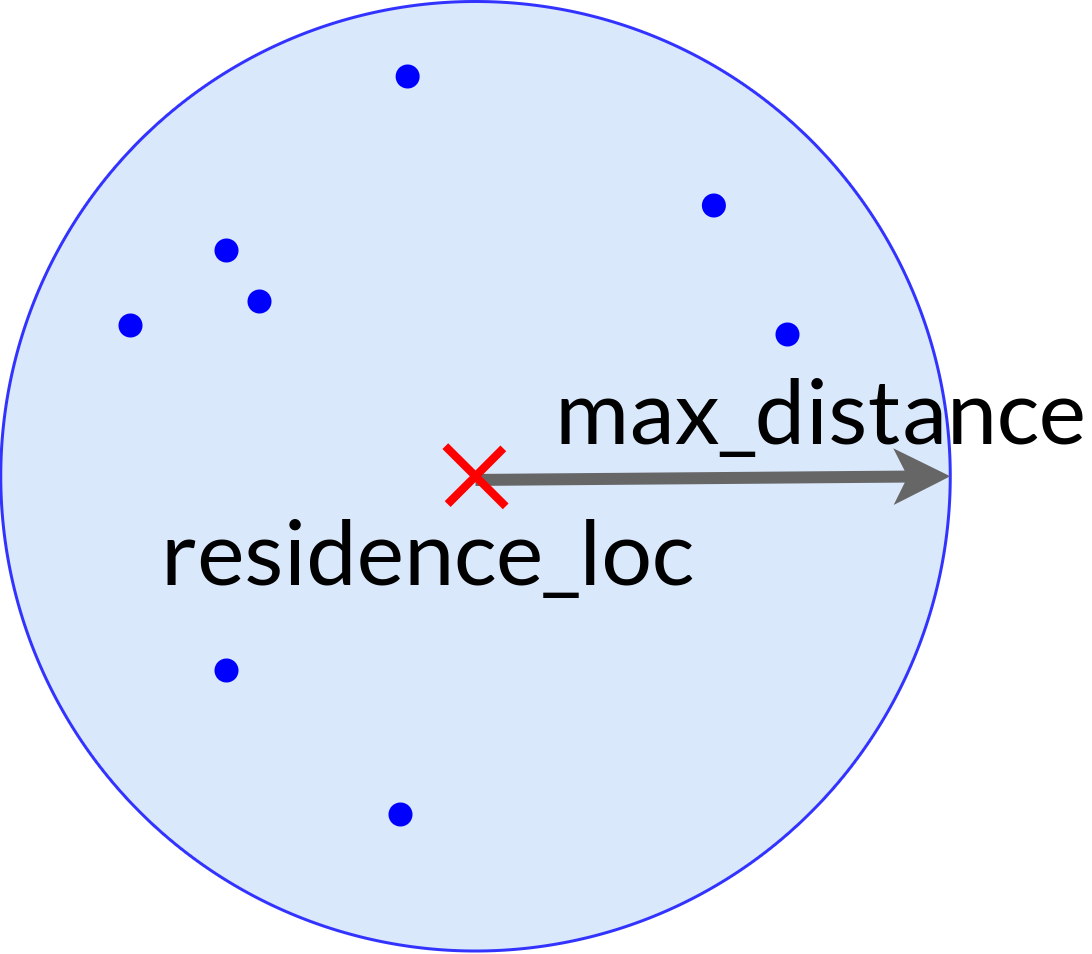
\includegraphics[scale=0.5]{images/tx-generation-tmin.png}
            \caption{\texttt{max\_distance} upper bound for the calculation of \texttt{t\_min}}
        \end{figure}    
          \item Specifically: Taking the specific maximum distance between all the ATM pairs 
          in the ATM subset to get the \textcolor{orange}{\texttt{t\_min}}.
      \end{itemize}  
      \item \texttt{max\_speed}: maximum speed at which it is possible to travel 
      (by any possible means of transport) between any pair of ATMs $\in 
      \ \texttt{Neighborhood}$.
    \end{itemize}

    \item For each day generate \textcolor{orange}{\texttt{num\_tx}} transactions, random 
    number drawn from a Poisson distribution of $\lambda = \texttt{withdrawal\_day}$.

    \item Distribution of the \texttt{num\_tx} transaction times 
    (\texttt{transaction\_start}), doing a uniform distribution of the \texttt{num\_tx}
    for each of the days: 
    
    We create an ordered list of  \texttt{num\_tx} start moments in seconds in a day 
    (in the range $[\texttt{t\_min}/2, 86400-(\texttt{t\_min}/2)-\texttt{max\_duration}]$) so that all of them are at a minimum time distance of $\texttt{t\_min} + \texttt{max\_duration}$. See Figure \ref{img:tx-distribution}.
    \textit{\texttt{max\_duration} limits the maximum duration of an ordinary transaction. 
    For the moment it was set to be of 10 minutes (600s)}.\\
    Note that the interval bounds for the transaction start moments are designed in such 
    a way that the \texttt{t\_min} minimum time distance between the end of a transaction 
    and the start of the next transaction is also respected between transactions belonging 
    to different consecutive days. See Figure \ref{img:tx-distribution-day}. 
    \textcolor{red}{Note that this way of generation (day by day) we are not allowing 
    transactions to occur in the interval marked among the two red dotted lines of the 
    Figure \ref{img:tx-distribution-day}.} \textcolor{orange}{NOTE/TODO: This could be 
    fixed by looking to the start time of the last transaction of the previous day...}. 
    The start moments are therefore taken to define the \texttt{transaction\_start} of 
    each of the transactions of that day. \texttt{transaction\_end} is assigned a shifted 
    time difference with the respective \texttt{transaction\_start}, in particular the 
    difference is drawn from a normal distribution $\mathcal{N}(300,\,120)$ that defines 
    the duration of a transaction to be of mean of 5 minutes (300s) and a standard 
    deviation of 2 minutes (120s), bounding it to be of a maximum time of 
    \texttt{max\_duration} of 10 minutes (600s) and setting it to the mean if the 
    distribution sample was negative. 

    \begin{figure}[H]
        \centering
        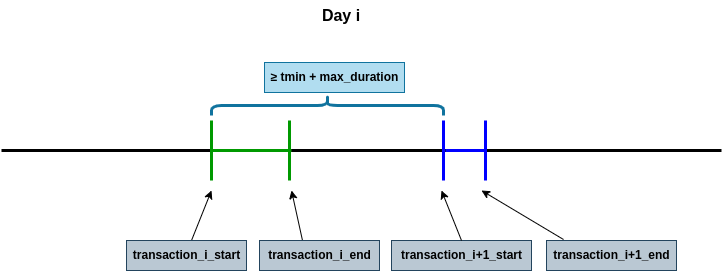
\includegraphics[scale = 0.45]{images/tx-distribution-1.png}
        \caption{Time distance limit between two consecutive transactions}
        \label{img:tx-distribution}
    \end{figure}
    \begin{figure}[H]
        \centering
        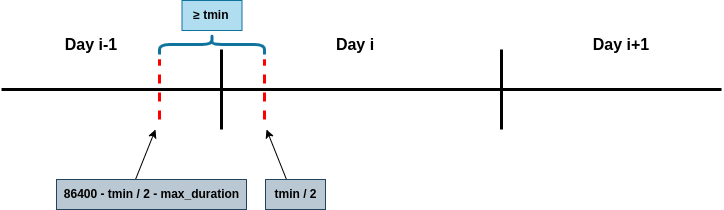
\includegraphics[scale = 0.45]{images/tx-distribution.png}
        \caption{Time distance limit between two consecutive transactions between two days}
        \label{img:tx-distribution-day}
    \end{figure}
    Note that a limit was set on the duration of the transaction so that we can have the 
    control avoiding time overlapping transactions, which will be producing irregular 
    undesired fraud pattern alerts.
    \item \texttt{transaction\_amount}: based on card behavior parameters, it is drawn 
    from a normal distribution
    $\mathcal{N}(\texttt{amount\_avg},\,\texttt{amount\_std})$. If negative amount, drawn 
    from a uniform distribution $\mathcal{U}(0,\ \texttt{amount\_avg}*2)$.
\end{itemize}

% --------------------------------------------------------------------------------------------------------------
% TODO: CONTINUE HERE 
Note that this approach is done with the focus on avoiding the production of potential
fraud scenarios. By taking into account the previous generated transaction: both for the
linked ATM of the new transaction and its transaction time (to avoid transactions that 
are overlapped or that come one directly after the other, since this may be fraudulent!).


\subsubsection{Poisson Process}



\subsubsection{Random Walk}



\end{document}
